\documentclass[twocolumn]{article}
\usepackage{listings}
\usepackage{graphicx}
\title{Lab#2\\Computational Physics I - Phys381}
\author{Guilherme Contesini 10140201 \\ Gerswin Magat 00325287}

\begin{document}

\maketitle

\newpage

%%%%%%%%%%%%%%%%%%%%%%%%%%%%%%%%%%%%%%%%%%%%%%%%%%%%%%%%%%%%%%%%%%%%%%%%%%%%%%%%%%%%%%%%%%%%%%%%%%%%%%%%%%%%%%%%%%%%%%%%

\section{1 - Fractals}

%%%%%%%%%%%%%%%%%%%%%%%%%%%%%%%%%%%%%%%%%%%%%%%%%%%%%%%%%%%%%%%%%%%%%%%%%%%%%%%%%%%%%%%%%%%%%%%%%%%%%%%%%%%%%%%%%%%%%%%%

\subsection{Question a:}
This function is a wave package in the interval x=[-4,4] when t = 0.
\begin{figure}[h!]

\begin{center}
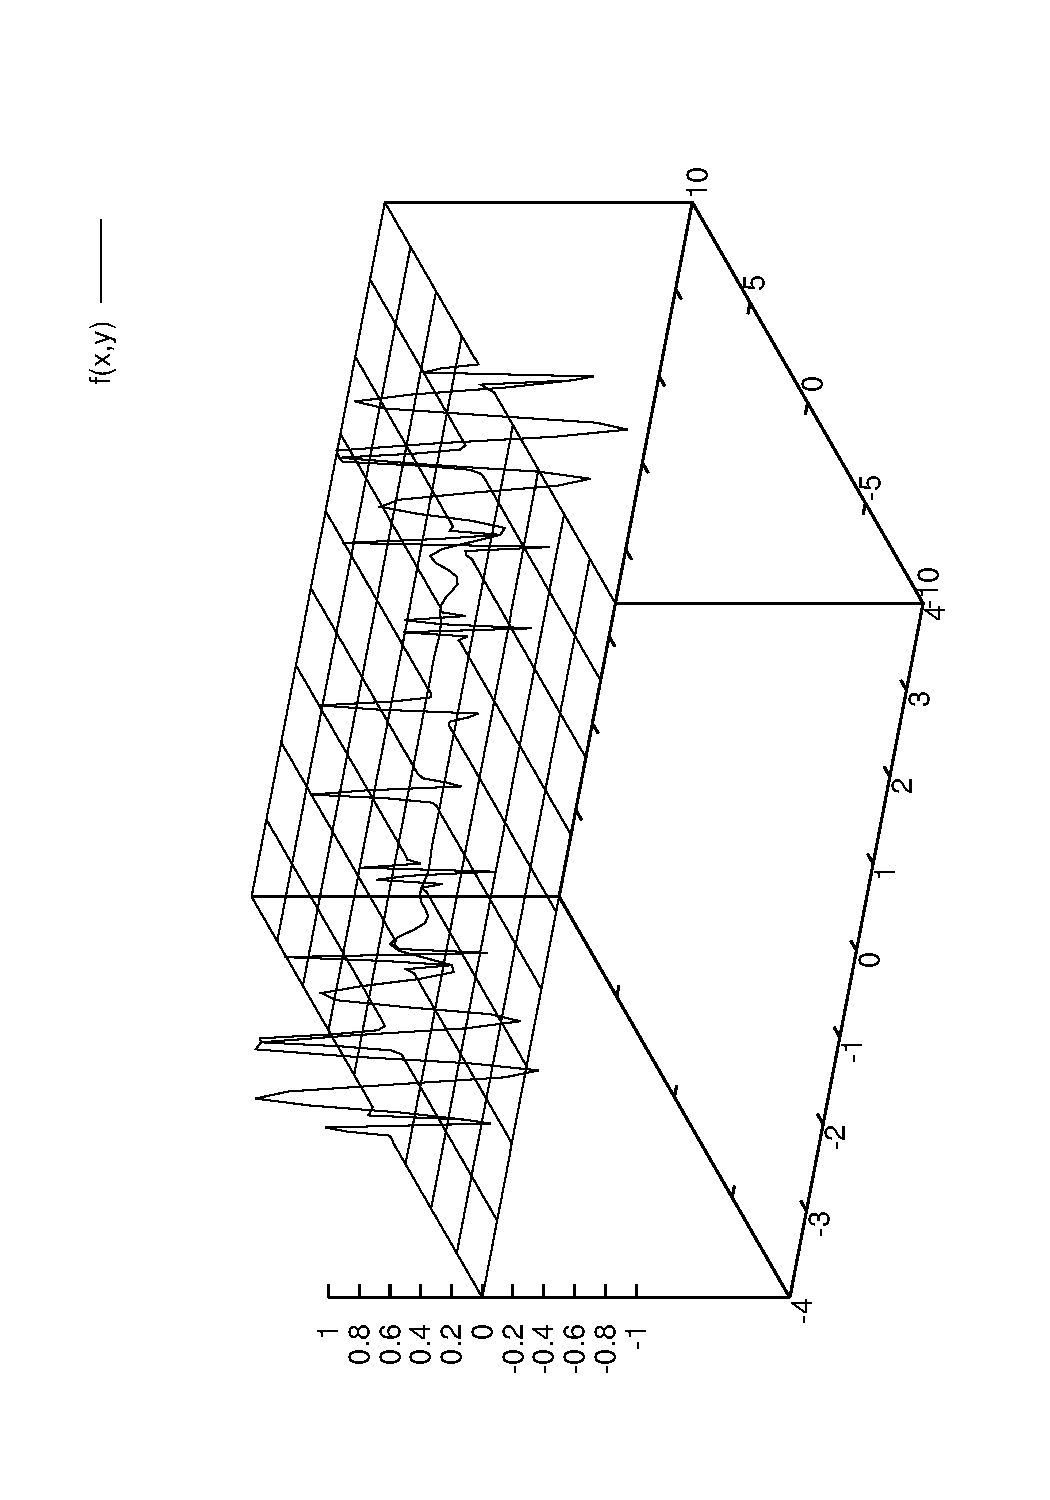
\includegraphics[width=2in,angle=270]{a.pdf}
\label{fig1}
\end{center}

\end{figure}

%%%%%%%%%%%%%%%%%%%%%%%%%%%%%%%%%%%%%%%%%%%%%%%%%%%%%%%%%%%%%%%%%%%%%%%%%%%%%%%%%%%%%%%%%%%%%%%%%%%%%%%%%%%%%%%%%%%%%%%%

\newpage

%%%%%%%%%%%%%%%%%%%%%%%%%%%%%%%%%%%%%%%%%%%%%%%%%%%%%%%%%%%%%%%%%%%%%%%%%%%%%%%%%%%%%%%%%%%%%%%%%%%%%%%%%%%%%%%%%%%%%%%%

\subsection{Question B:}
These 3 graphics show the same function at times: t=-1,0,+1.
\begin{figure}[h!]

\begin{center}
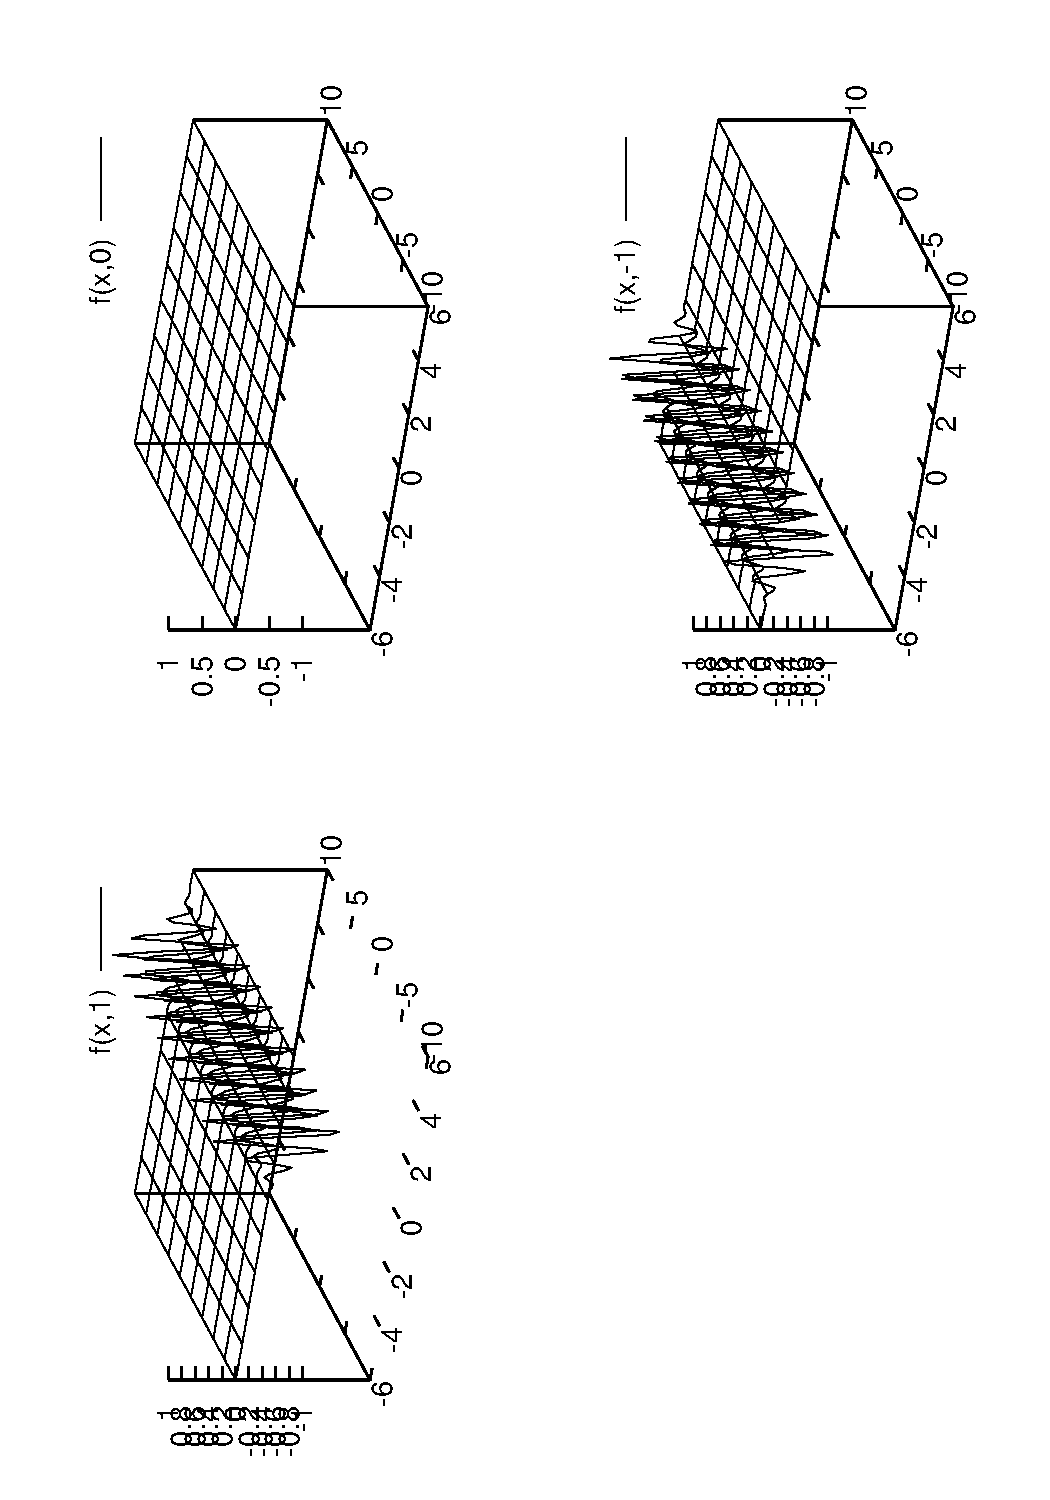
\includegraphics[width=2in,angle=270]{b.pdf}
\label{fig2}
\end{center}

\end{figure}

%%%%%%%%%%%%%%%%%%%%%%%%%%%%%%%%%%%%%%%%%%%%%%%%%%%%%%%%%%%%%%%%%%%%%%%%%%%%%%%%%%%%%%%%%%%%%%%%%%%%%%%%%%%%%%%%%%%%%%%%

\newpage

%%%%%%%%%%%%%%%%%%%%%%%%%%%%%%%%%%%%%%%%%%%%%%%%%%%%%%%%%%%%%%%%%%%%%%%%%%%%%%%%%%%%%%%%%%%%%%%%%%%%%%%%%%%%%%%%%%%%%%%%

\subsection{Question C:}
This picture is a two-dimensional surface plot of the function f(x,y) in the intervals x=[-6,6] and t=[-1,1]
\begin{figure}[h!]

\begin{center}
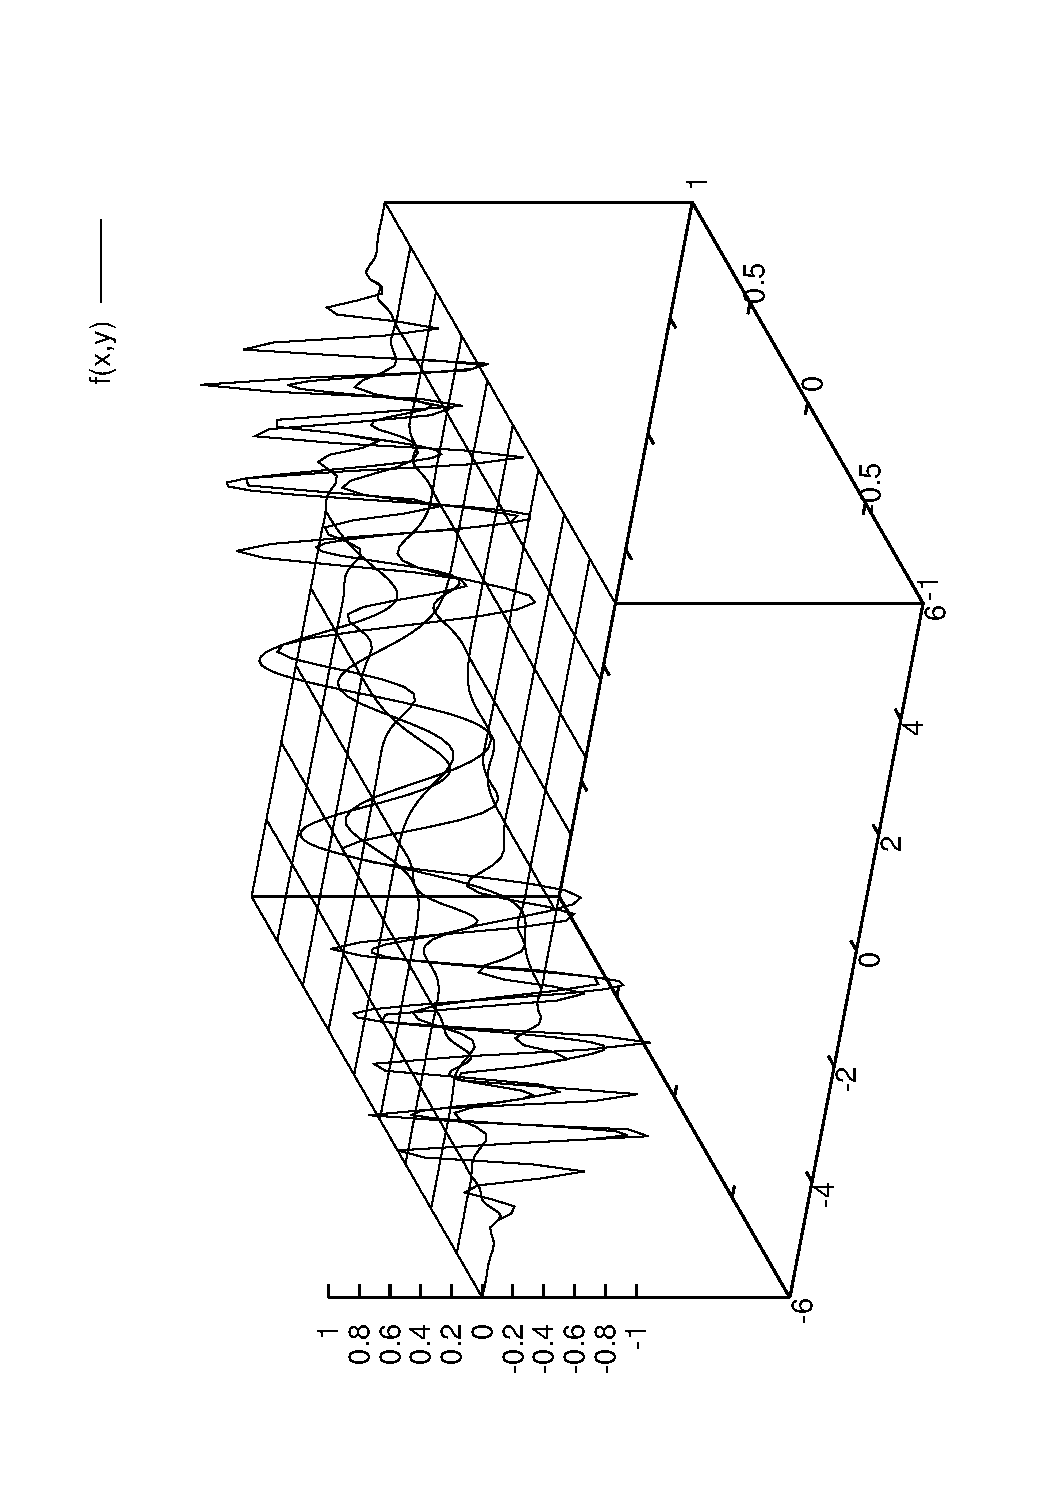
\includegraphics[width=2in,angle=270]{c.pdf}
\label{fig3}
\end{center}

\end{figure}

%%%%%%%%%%%%%%%%%%%%%%%%%%%%%%%%%%%%%%%%%%%%%%%%%%%%%%%%%%%%%%%%%%%%%%%%%%%%%%%%%%%%%%%%%%%%%%%%%%%%%%%%%%%%%%%%%%%%%%%%

\subsection{Question D:}
This animation shows the wave moving to the right. the velocity of the waves and the packet is different. This can help visualizing multiple waves and their interactions with each other.

%%%%%%%%%%%%%%%%%%%%%%%%%%%%%%%%%%%%%%%%%%%%%%%%%%%%%%%%%%%%%%%%%%%%%%%%%%%%%%%%%%%%%%%%%%%%%%%%%%%%%%%%%%%%%%%%%%%%%%%%

\subsection{Codes:}

\begin{listing}
\begin{indent}
\\
Question a:
\\
\\
set terminal postscript
\\
set output "a.eps"
\\
f(x,y)=exp(-(x-3*y)**2)*sin(3*3.14*(x*y))
\\
set xrange[-4:4]
\\
splot f(x,y)
\\
!epstopdf "a.eps" && rm "a.eps"
\end{indent}
\end{listing}
\\
\\
%%%%%%%%%%%%%%%%%%%%%%%%%%%%%%%%%%%%%%%%%%%%%%%%%%%%%%%%%%%%%%%%%%%%%%%%%%%%%%%%%%%%%%%%%%%%%%%%%%%%%%%%%%%%%%%%%%%%%%%%

%%%%%%%%%%%%%%%%%%%%%%%%%%%%%%%%%%%%%%%%%%%%%%%%%%%%%%%%%%%%%%%%%%%%%%%%%%%%%%%%%%%%%%%%%%%%%%%%%%%%%%%%%%%%%%%%%%%%%%%%
\begin{listing}
\begin{indent}
\\
Question b:
\\
\\
set terminal postscript
\\
set output "b.eps"
\\
set multiplot
\\
f(x,y) = exp(-(x-3*y)**2)*sin(3*3.14*(x*y))
\\
set size 0.5,0.5
\\
set xrange[-6:6]
\\
set origin 0.5 , 0.0
\\
splot f(x,-1)
\\
set origin 0.5 , 0.5
\\
splot f(x,0)
\\
set origin 0.0 , 0.5
\\
splot f(x,1)
\\
!epstopdf "b.eps" && rm "b.eps"
\\
unset multiplot
\\
reset
\end{indent}
\end{listing}

%%%%%%%%%%%%%%%%%%%%%%%%%%%%%%%%%%%%%%%%%%%%%%%%%%%%%%%%%%%%%%%%%%%%%%%%%%%%%%%%%%%%%%%%%%%%%%%%%%%%%%%%%%%%%%%%%%%%%%%%

\\
\\

%%%%%%%%%%%%%%%%%%%%%%%%%%%%%%%%%%%%%%%%%%%%%%%%%%%%%%%%%%%%%%%%%%%%%%%%%%%%%%%%%%%%%%%%%%%%%%%%%%%%%%%%%%%%%%%%%%%%%%%%

\begin{listing}
\begin{indent}
\\
Question c:
\\
\\
set terminal postscript
\\
set output "c.eps"
\\
f(x,y) = exp(-(x-3*y)**2)*sin(3*3.14*(x*y))
\\
set xrange[-6:6]
\\
set yrange[-1:1]
\\
splot f(x,y)
\\
!epstopdf "c.eps" && rm "c.eps"
\end{indent}
\end{listing}

%%%%%%%%%%%%%%%%%%%%%%%%%%%%%%%%%%%%%%%%%%%%%%%%%%%%%%%%%%%%%%%%%%%%%%%%%%%%%%%%%%%%%%%%%%%%%%%%%%%%%%%%%%%%%%%%%%%%%%%%

\end{document}